\newcommand{\FigICEDUSTOverview}{
\begin{figure}[t]
\centering
%\fbox{
\includegraphics[width=1.00\textwidth,trim=0.85cm 0.5cm 0.5cm 0.5cm,clip=true]{figs/software/ICEDUST_structure}
%}
\caption{
Overview diagram for the ICEDUST framework.
Data produced from simulation or taken in the real experiment are treated identically through the calibration and onwards up to analysis.
}
\figlabel{software:ICEDUSTOverview}
\end{figure}
}

\newcommand{\FigNDTwoEighty}{
\begin{figure}[t]
\centering
\includegraphics[width=0.95\textwidth]{figs/software/ND280SoftwareDiagram}
\caption{
Overview diagram for the ND280 framework.
}
\figlabel{software:ND280}
\end{figure}
}

\newcommand{\FigSimulationOverview}{
\begin{figure}[t]
\centering
%\fbox{
\includegraphics[width=1.00\textwidth]{figs/software/Simulation_structure}
%}
\caption{
Diagram showing the stages used to simulate COMET.
The timing schematics on the right show how a simulated event is built up, firstly by producing many individual proton interactions with the production target,
then by transporting the secondary particles to produce energy deposits in the detector, which are then combined with the truth hits from other proton events to produce a realistic bunch structure.
Finally, these bunch events are processed through the detector response simulation to produce fake waveforms and other detector read-outs.
}
\figlabel{software:SimulationOverview}
\end{figure}
}

\newcommand{\FigGeometryHeirarchy}{
\begin{figure}[t]
\centering
%\fbox{
\includegraphics[width=0.70\textwidth]{figs/software/ComponentHeirarchy}
%}
\caption{
How parameters are shared amongst different components.
Parameters of component 1.a (in red) can access the value of parameters owned by components contained in the larger violet region.
}
\figlabel{software:componentHeirarchy}
\end{figure}
}

\newcommand{\FigGeometryParameters}{
\begin{figure}[t]
\lstinputlisting[style=customc]{figs/software/demo-parameters.mac}
\caption{
An example set of parameter definitions which control the geometry for the Torus2.
Parameter specifications use natural arithmetic notation and can reference other parameters and use standard units.
They can also be formed as sets where each element has a different value, such as the \texttt{Coils:Position} parameter.
}
\figlabel{software:geom:paramAssignments}
\end{figure}
}

\newcommand{\FigGeometryScreenshots}{
\begin{figure}[tb]
        \subfloat[][\figlabel{software:geom:screenshots:phaseI}\phaseI]  {\includegraphics[height=0.25\textheight]{figs/software/Phase-I-UpdateGeom}}\hspace{2ex}%
        \subfloat[][\figlabel{software:geom:screenshots:phaseII}\phaseII]{\includegraphics[height=0.25\textheight,trim=0 0.3cm 0 2.6cm,clip=true]{figs/software/Phase-II-UpdateGeom.png}}
\caption{\figlabel{software:geom:screenshots} %
Two of the possible simulation `worlds' that can be selected at run-time:
        \protect\subref{fig:software:geom:screenshots:phaseI} \phaseI with the CyDet detector installed, and
        \protect\subref{fig:software:geom:screenshots:phaseII} \phaseII.  
	Mutiple \phaseI worlds exist, one for each potential running configuration.
}
\end{figure}
}

\newcommand{\FigPiYieldHadronCodes}{
\begin{figure}[b]
\centering
%\fbox{
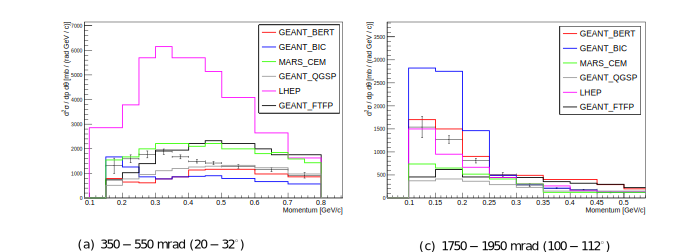
\includegraphics[width=0.95\textwidth,trim=2cm 1cm 0.8cm 0.5cm,clip=true]{figs/software/PionYield_AEdmondsThesis}
%}
\caption{
Comparison of various hadron production codes with experimental data from the HARP experiment, taken from the thesis of A. Edmonds~\cite{AEdmondsThesis}.
Points with error bars are the experimental data.  Left: double differential-production cross-section for pion production from 20 to 32\degree with respect to the incoming proton direction; right: from 100 to 112\degree.
The hadron production code that best reproduces the data depends strongly on the angular region under consideration.
}
\figlabel{software:piYield}
\end{figure}
}

\newcommand{\FigSoftwarePhysicsSpectra}{
\begin{figure}[p]
\centering
%\fbox{
\subfloat[][\figlabel{software:customPhysic:DIO}Electrons from $\mu$ Decay-in-Orbit]{
\includegraphics[width=0.45\textwidth,trim=0cm 0cm 0.0cm 1.3cm,clip=true]{figs/software/160822_BoundDecay_Geant4_vs_Czarnecki-lin.pdf}
\includegraphics[width=0.45\textwidth,trim=0cm 0cm 0.0cm 1.3cm,clip=true]{figs/software/160822_BoundDecay_Geant4_vs_Czarnecki-log.pdf}
}\\
\subfloat[][\figlabel{software:customPhysic:ProtMuCap}Protons Emitted Following $\mu$ Nuclear Capture]{
\includegraphics[width=0.45\textwidth,trim=0cm 0cm 1.8cm 1.9cm,clip=true]{figs/software/160822_Geant4VsAlcap-lin.pdf}
\includegraphics[width=0.45\textwidth,trim=0cm 0cm 1.8cm 1.9cm,clip=true]{figs/software/160822_Geant4VsAlcap-log.pdf}
}
%}
\caption{
\figlabel{software:customPhysic}
Comparison of the realistic spectra for \ac{DIO} electrons, \protect\subref{fig:software:customPhysic:DIO} (normalised to agree at 35~MeV), and protons coming from muon nuclear capture, \protect\subref{fig:software:customPhysic:ProtMuCap} (normalised to have the same maximum value), each on a linear scale (left) and a logarithmic scale (right).
The \ac{DIO} spectrum used in default Geant4 has a sharp cut-off slightly above the free muon decay end-point, to be compared with the long but steeply falling tail of the Czarnecki \etal theoretical calculation~\cite{Czarnecki2011}.
The comparison of protons coming from muon capture between the preliminary result from AlCap and default Geant4 shows that the true proton spectrum is much softer than the Geant4 model.
}
\end{figure}
}

\newcommand{\FigSimulationPhysicsClasses}{
\begin{figure}[tb]
\centering
%\fbox{
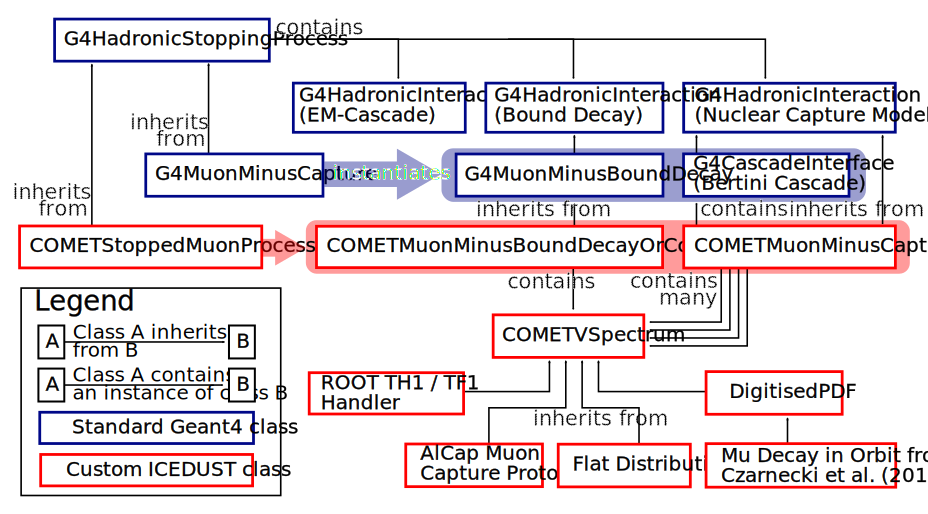
\includegraphics[width=1.00\textwidth]{figs/software/SimulationMuonPhysicsClasses}
%}
\caption{
The various classes involved in simulating the various processes of stopped negative muons.
%Classes in red have been implemented for COMET and augment the existing Geant4 classes which are shown in blue.
The standard Geant4 model is activated by registering `G4MuonMinusCapture', which instantiates `G4MuonMinusBoundDecay' and `G4CascadeInterface' to run the \ac{DIO} and nuclear capture respectively.
To use the custom COMET muon physics, an instance of `COMETStoppedMuonProcess' should be registered, which sets up `COMETMuonMinusBoundDecayOrConversion' to produce the electron (and possibly neutrinos) from \ac{DIO} or conversion, and `COMETMuonMinusCapture' to do the nuclear capture.
}
\figlabel{software:ExtendedMuonClasses}
\end{figure}
}

\newcommand{\FigSoftwareFieldMap}{
\begin{figure}[b]
\centering
%\fbox{
\subfloat[][\figlabel{software:field:Opera}Opera calculation]{
\includegraphics[width=0.45\textwidth,trim=0cm 0cm 0.0cm 13cm,clip=true]{figs/software/Plot_Opera.png}
}
\subfloat[][\figlabel{software:field:G4Beamline}G4Beamline calculation]{
\includegraphics[width=0.45\textwidth,trim=0cm 0cm 0.0cm 13cm,clip=true]{figs/software/Plot_G4Beamline.png}
}
%}
\caption{
\figlabel{software:field}
Fieldmap produced by \protect\subref{fig:software:field:Opera} Opera and \protect\subref{fig:software:field:G4Beamline} G4Beamline.
Although the fringe field is larger with the G4Beamline calculation, the lack of material effects make this calculation less reliable.
Note that the G4Beamline calculation does not include the detector solenoid.
}
\end{figure}
}

\newcommand{\FigSoftwareFieldMapComparison}{
\begin{figure}[t]
\centering
%\fbox{
\includegraphics[width=0.9\textwidth,trim=0cm 0cm 0.0cm 13cm,clip=true]{figs/software/Plot_ratio_opera-G4Beamline.png}
%}
\caption{
\figlabel{software:field:comparison}
The ratio of the Opera and G4Beamline calculations shown in \fig{software:field}.
For most of the field within the beamline the calculations agree within 10\%, although around the ends of the solenoids the agreement is poorer.
}
\end{figure}
}

\newcommand{\FigSoftwareDipoleField}{
\begin{figure}[t]
\centering
%\fbox{
\includegraphics[width=0.9\textwidth,trim=2cm 8cm 0.0cm 6cm,clip=true]{figs/software/DipoleFields.png}
%}
\caption{
\figlabel{software:field:dipole}
The dipole field calculations used in ICEDUST for \phaseII. 
Three dipole fields are applied in COMET, one over each of the Torus1, Torus2 and the Electron Spectrometer.
The dipoles over the bent muon transport beamline point in the opposite direction to that over the electron spectrometer.
It can also be seen that the calculation for the dipole along the muon transport beamline contains realistic features (fringe fields, non-uniformities, etc)
whilst the dipole field for the electron spectrometer is artificially uniform.  
}
\end{figure}
}

\newcommand{\FigSoftwareBeamline}{
\begin{figure}[t]
\centering
\subfloat[][\figlabel{software:beamline:dist}Beamline Distance]{
%\fbox{
\includegraphics[width=0.45\textwidth,trim=1cm 4cm 0.0cm 4.5cm,clip=true]{figs/software/BeamlineCoords_longitudinal.png}
}
\subfloat[][\figlabel{software:beamline:horiz}Horizontal Beamline Component]{
\includegraphics[width=0.45\textwidth,trim=1cm 4cm 0.0cm 4.5cm,clip=true]{figs/software/BeamlineCoords_horizontal.png}
}
%}
\caption{
\figlabel{software:beamline}
	The longitudinal \protect\subref{fig:software:beamline:dist} and horizontal \protect\subref{fig:software:beamline:horiz} components of the beamline coordinate system for different points in the global X-Z plane.
	Although this image shows the \phaseI geometry, the implementation in ICEDUST will semi-automatically adjust to whatever geometry was used.
}
\end{figure}
}

\newcommand{\FigSoftwareBeamlineAnalysis}{%
\begin{figure}[bt]
\centering 
\subfloat[\figlabel{software:beamline:analysis:height}Two-dimensional flux]{
	\includegraphics[width=0.8\textwidth,trim=8.3cm 1.5cm 13.2cm 2.2cm,clip]{figs/sensitivity/Tidied_SignalHeight2DVsBeamline.png}}\\
\subfloat[\figlabel{software:beamline:analysis:flux}One-dimensional flux]{
        \includegraphics[width=0.8\textwidth,trim=1.0cm 0.2cm 1.7cm 0.4cm,clip]{figs/sensitivity/Tidied_SignalSurivivalVsBeamline.pdf}}
\caption{\figlabel{software:beamline:analysis}
Different flux plots that make use of the beamline coordinate system.
\protect\subref{fig:sense:accept:height} Projection of trajectories onto the vertical-beamline axis plane.  Setting a limit to the maximum step size forces Geant4 to create steps with more regular interval.
Each step is then projected to the vertical-beamline surface, such that the density of points represents the flux of particles.
\protect\subref{fig:sense:accept:flux} A one dimensional flux plot, where every bin between the beginning and end of a particle's track is filled.
}
\end{figure}\xspace}

